\documentclass[11pt,a4paper]{article}
\usepackage[margin=18mm,top=22mm,bottom=20mm]{geometry}
\usepackage{fontspec}\setmainfont{Latin Modern Roman}
\usepackage{amsmath,amssymb,tikz,graphicx,fancyhdr,array,needspace}
\usetikzlibrary{patterns,arrows.meta,decorations.pathmorphing,calc}
\setlength{\headheight}{14pt}
\usetikzlibrary{arrows.meta}
\pagestyle{fancy}\fancyhf{}\renewcommand{\headrulewidth}{0.4pt}
\fancyhead[L]{\textbf{M-06}}\fancyhead[C]{\itshape Fizika (OliyFizika.uz mock test)}\fancyhead[R]{\textbf{Mock №6}}
\fancyfoot[C]{\thepage}
\setlength{\parindent}{0pt}\setlength{\parskip}{3pt}
\newcommand{\opt}[2]{\hspace*{4mm}#1)\ #2\par}
\newcommand{\blank}{\rule{5cm}{0.4pt}}
\begin{document}

\begin{center}{\Large\textbf{FIZIKA}}\end{center}
\noindent\begin{minipage}{\linewidth}
\textbf{1.}\ Muz ustida 80 kg massali odam 16 kg massali yukni sirpantirib yubordi. Yuk 4 s da 15 m masofa yurib töxtagan bölsa, odamning olgan eng katta kinetik energiyasini (J) hisoblang.\par\smallskip
\opt{A}{30}
\opt{B}{60}
\opt{C}{120}
\opt{D}{90}
\end{minipage}\vspace{9pt}\par
\noindent\begin{minipage}{\linewidth}
\textbf{2.}\ Sun’iy yöldoş orbitasining diametri 2 marta ortganda uning tezligi qanday özgaradi?\par\smallskip
\opt{A}{2 marta ortadi}
\opt{B}{2 marta kamayadi}
\opt{C}{$\sqrt2$ marta ortadi}
\opt{D}{$\sqrt2$ marta kamayadi}
\end{minipage}\vspace{9pt}\par
\noindent\begin{minipage}{\linewidth}
\textbf{3.}\ $m$ massali, $l$ uzunlikli sterjen tik holda suvda suzib yuribdi, uning suv içidagi qismi $0{,}8l$. Sterjenni tik holda suvga töliq botiriş uçun zarur bölgan minimal energiya hisoblansin.\par\smallskip
\opt{A}{$mgl/45$}
\opt{B}{$mgl/37$}
\opt{C}{$mgl/42$}
\opt{D}{$mgl/40$}
\end{minipage}\vspace{9pt}\par
\noindent\begin{minipage}{\linewidth}
\textbf{4.}\ Töğri çiziqli tekis tezlanuvçan harakatlanayotgan jism birinçi sekundda 1 m, ikkinçi sekundda – 2 m, uçinçi sekundda – 3 m masofani ötadi. Jismning boşlanğiç tezligini aniqlang (m/s).\par\smallskip
\opt{A}{0}
\opt{B}{1,5}
\opt{C}{1}
\opt{D}{0,5}
\end{minipage}\vspace{9pt}\par
\noindent\begin{minipage}{\linewidth}
\textbf{5.}\ Quyoşning umumiy nurlaniş quvvati 3,83$\cdot10^{6}$ W. Şu tufayli Quyoş massasi har sekundda qançaga kamayadi (kg)?\par\smallskip
\opt{A}{3,5$\cdot10^{9}$}
\opt{B}{4$\cdot10^{9}$}
\opt{C}{4,3$\cdot10^{-9}$}
\opt{D}{4,5$\cdot10^{-9}$}
\end{minipage}\vspace{9pt}\par
\noindent\begin{minipage}{\linewidth}
\textbf{6.}\ Qanday holatda gazni suyuqlikka aylantiriş mumkin?\par\smallskip
\opt{A}{bosim kritik qiymatdan yuqori, temperatura esa kritik qiymatdan past}
\opt{B}{bosim kritik qiymatdan past, temperatura esa kritik qiymatdan yuqori bölganda}
\opt{C}{bosim kritik qiymatdan yuqori, temperatura esa kritik qiymatdan katta bölganda}
\opt{D}{bosim kritik qiymatdan past, temperatura esa kritik qiymatdan kam bölganda}
\end{minipage}\vspace{9pt}\par
\noindent\begin{minipage}{\linewidth}
\textbf{7.}\ Örtaça tezligi 20 m/s bölgan jism 6 s da qança masofa (m) bosadi?\par\smallskip
\opt{A}{60}
\opt{B}{20}
\opt{C}{120}
\opt{D}{40}
\end{minipage}\vspace{9pt}\par
\noindent\begin{minipage}{\linewidth}
\textbf{8.}\ Moddiy nuqta tekislikda özaro perpendikulyar bölgan ikkita garmonik harakatda iştirok etmoqda. Ularning davrlari mos holda 1 s va 2 s. t=5 s paytda moddiy nuqta muvozanat nuqtasidan ötdi. Qanday t vaqtda (s) moddiy nuqta muvozanat nuqtasiga ikkinçi marta qaytib keladi?\par\smallskip
\opt{A}{11}
\opt{B}{6}
\opt{C}{17}
\opt{D}{12}
\end{minipage}\vspace{9pt}\par
\noindent\begin{minipage}{\linewidth}
\textbf{9.}\ Vodorod bilan töldirilgan bolalar şarining hajmi 3 l, oğirligi esa 0,034 N. U qanday oğirlikdagi yukni kötara oladi (mN)? Havoning ziçligi 1,29 kg/m$^{3}$. g=10 N/kg.\par\smallskip
\opt{A}{4,7}
\opt{B}{31,3}
\opt{C}{36,7}
\opt{D}{72}
\end{minipage}\vspace{9pt}\par
\noindent\begin{minipage}{\linewidth}
\textbf{10.}\ Ikkita moddiy nuqta $x_1=3\sin(\pi t+2\pi)$ [m] va $x_2=3\sin(2\pi t-\pi)$ [m] qonunlarga köra garmonik tebranmoqda. Qança vaqtdan keyin nuqtalarning tebraniş fazalari özaro tenglaşadi (s)?\par\smallskip
\opt{A}{1}
\opt{B}{2}
\opt{C}{4}
\opt{D}{3}
\end{minipage}\vspace{9pt}\par
\noindent\begin{minipage}{\linewidth}
\textbf{11.}\ Agar har 10 m balandlikda atmosfera bosimi 1 mm.Hg ga kamayadigan bölsa, dengiz sathidan 4,6 km balandlikdagi havoning 1 cm$^{3}$ hajmida qança molekula böladi? Dengiz sathida atmosfera bosimi 760 mm.Hg ga teng. Havo harorati 27 $^\circ$C. Haroratning balandlik böyiça özgarişini hisobga olmang. 1 mm.Hg=133,3 Pa.\par\smallskip
\opt{A}{9,66$\cdot10^{17}$}
\opt{B}{4,66$\cdot10^{15}$}
\opt{C}{9,66$\cdot10^{20}$}
\opt{D}{9,66$\cdot10^{18}$}
\end{minipage}\vspace{9pt}\par
\noindent\begin{minipage}{\linewidth}
\textbf{12.}\ Ideal gazning hajmi $V$ ga, konsentratsiyasi $n$ ga teng. Agar har bir gaz molekulasi örtaça $\bar{E}_k$ kinetik energiyaga ega bölsa, gazning içki energiyasini aniqlang.\par\smallskip
\opt{A}{$\dfrac{\bar{E}_k}{nV}$}
\opt{B}{$nV\bar{E}_k$}
\opt{C}{$\dfrac{V\bar{E}_k}{n}$}
\opt{D}{$\dfrac{n\bar{E}_k}{V}$}
\end{minipage}\vspace{9pt}\par
\noindent\begin{minipage}{\linewidth}
\textbf{13.}\ 44 g karbonat angidriddagi molekulalar soniga..... deb ataladi.\par\smallskip
\opt{A}{atom massa}
\opt{B}{konsentratsiya}
\opt{C}{molyar massa}
\opt{D}{Avogadro soni}
\end{minipage}\vspace{9pt}\par
\noindent\begin{minipage}{\linewidth}
\textbf{14.}\ Elektr yurituvçi kuçi 2 V, içki qarşiligi 2 $\Omega$ bölgan manbaga şunday qarşilik ulandiki, bunda undagi quvvat maksimal qiymatga erişdi. Uşbu quvvatni toping (W). Manbaning F.I.K ni toping (\%).\par\smallskip
\opt{A}{0,6; 50}
\opt{B}{0,2; 40}
\opt{C}{0,5; 50}
\opt{D}{1; 50}
\end{minipage}\vspace{9pt}\par
\noindent\begin{minipage}{\linewidth}
\textbf{15.}\ Temperaturasi 5 $^\circ$C va massasi 2 kg bölgan suvga 2 kg massali 0 $^\circ$C dagi muz solindi. Qaror topgan temperaturani toping (K). c=4200 J/kg$\cdot$K, $\lambda$=330 kJ/kg.\par\smallskip
\opt{A}{0}
\opt{B}{273}
\opt{C}{273,8}
\opt{D}{2,85}
\end{minipage}\vspace{9pt}\par
\noindent\begin{minipage}{\linewidth}
\textbf{16.}\ Özgarmas tok manabaining qutblaridagi kuçlaniş qanday holatda maksimal darajada böladi?\par\smallskip
\opt{A}{qisqa tutaşuvda}
\opt{B}{taşqi zanjir berkitilmaganda}
\opt{C}{taşqi zanjir berkitilganda}
\opt{D}{taşqi qarşilik içki qarşilikka teng bölganda}
\end{minipage}\vspace{9pt}\par
\noindent\begin{minipage}{\linewidth}
\textbf{17.}\ Ötkazgiçning uzunligi 800 m, undagi barça erkin elektronlarning umumiy impulsi $2\cdot10^{-7}$ kg$\cdot$m/s. Ötkazgiçdagi tok kuçi (A) topilsin. Elektron uçun $e/m$=$1{,}76\cdot10^{11}$ C/kg.\par\smallskip
\opt{A}{44}
\opt{B}{70}
\opt{C}{59}
\opt{D}{50}
\end{minipage}\vspace{9pt}\par
\noindent\begin{minipage}{\linewidth}
\textbf{18.}\ $\pi$ sekundda 1,25$\cdot10^{6}$ ta tebraniş yuzaga keluvçi tebranişlar konturida kondensator siğimi 16 nF bölsa, ğaltak induktivligini toping (mH).\par\smallskip
\opt{A}{0,02}
\opt{B}{0,2}
\opt{C}{0,1}
\opt{D}{0,01}
\end{minipage}\vspace{9pt}\par
\noindent\begin{minipage}{\linewidth}
\textbf{19.}\ Massalari $m$ dan bölgan $q$ va $3q$ zaryadli zarralar bir biridan $a$ masofada uşlab turilibdi. $q$ zaryadli zarra böşatib yuborilsa, u qanday maksimal tezlikka erişadi?\par\smallskip
\opt{A}{$\sqrt{\dfrac{3q^2}{am}}$}
\opt{B}{$\sqrt{\dfrac{6kq^2}{am}}$}
\opt{C}{$\sqrt{\dfrac{12kq}{am}}$}
\opt{D}{$\sqrt{\dfrac{18kq}{am}}$}
\end{minipage}\vspace{9pt}\par
\noindent\begin{minipage}{\linewidth}
\textbf{20.}\ Özgarmas tok manbaiga ulangan yassi kondensatorning yuzasi 3 marta orttirilsa, uning qoplamalari orasidagi elektr maydon energiya ziçligi qanday özgaradi?\par\smallskip
\opt{A}{özgarmaydi}
\opt{B}{3 marta ortadi}
\opt{C}{3 marta kamayadi}
\opt{D}{9 marta ortadi}
\end{minipage}\vspace{9pt}\par
\noindent\begin{minipage}{\linewidth}
\textbf{21.}\ Kondensatorining siğimi 4 marta ortsa, ideal tebraniş konturidagi erkin elektromagnit tebranişlar davri qanday özgaradi?\par\smallskip
\opt{A}{4 marta ortadi}
\opt{B}{2 marta kamayadi}
\opt{C}{2 marta ortadi}
\opt{D}{4 marta kamayadi}
\end{minipage}\vspace{9pt}\par
\noindent\begin{minipage}{\linewidth}
\textbf{22.}\ Özgaruvçan tok liniyasida kuçlaniş neça marta oşirilsa, liniyadagi energiya yöqotilişi 16 marta kamayadi?\par\smallskip
\opt{A}{5}
\opt{B}{2}
\opt{C}{4}
\opt{D}{8}
\end{minipage}\vspace{9pt}\par
\noindent\begin{minipage}{\linewidth}
\textbf{23.}\ Radiusi 5 cm bölgan sim halqa induksiyasi 0,2 T bo’lgan bir jinsli magnit maydonda joylaşgan. Agar halqadan 2 A özgarmas tok ötayotgan bölsa, magnit maydoni tomonidan unga qanday kuç momenti ta’sir etadi (N$\cdot$m)?\par\smallskip
\opt{A}{6,28$\cdot10^{-6}$}
\opt{B}{3,14$\cdot10^{-6}$}
\opt{C}{3,14$\cdot10^{-3}$}
\opt{D}{3,14}
\end{minipage}\vspace{9pt}\par
\noindent\begin{minipage}{\linewidth}
\textbf{24.}\ Yassi kondensator manbadan uzildi va qoplamalar orasidagi masofa 3 marta kamaytirildi. Bunda kondensatorning energiyasi qanday özgaradi?\par\smallskip
\opt{A}{3 marta ortadi}
\opt{B}{3 marta kamayadi}
\opt{C}{9 marta kamayadi}
\opt{D}{9 marta ortadi}
\end{minipage}\vspace{9pt}\par
\noindent\begin{minipage}{\linewidth}
\textbf{25.}\ E.Yu.K E=3,5 V va içki qarşiligi r=1,4 $\Omega$ bölgan 7 ta tok manbai özaro parallel ulanib batareya hosil qilindi. Batareyaga qarşiligi R (R \textgreater{} r) bölgan rezistor ulanganda 3,3 W foydali quvvat ajraldi. Zanjirdagi töla tok kuçi (A) qanday?\par\smallskip
\opt{A}{5}
\opt{B}{2}
\opt{C}{1}
\opt{D}{3,4}
\end{minipage}\vspace{9pt}\par
\noindent\begin{minipage}{\linewidth}
\textbf{26.}\ Yassi közgu va odam orasidagi masofa 4 m ga teng. Odam közgudan 1 m ga uzoqlaşdi. Közgu ham xuddi şu yönalişda 2 m ga surildi. Odam va uning tasviri orasidagi masofa qanday bölib qoladi (m)?\par\smallskip
\opt{A}{8}
\opt{B}{3}
\opt{C}{4}
\opt{D}{6}
\end{minipage}\vspace{9pt}\par
\noindent\begin{minipage}{\linewidth}
\textbf{27.}\ Optik kuçi 6 dptr bölgan yiğuvçi linza yordamida ekranda buyumning 2 marta kiçiklaşgan haqiqiy tasviri hosil qilindi. Buyum va tasvir orasidagi masofani (m) aniqlang\par\smallskip
\opt{A}{1/2}
\opt{B}{3/4}
\opt{C}{2}
\opt{D}{1/4}
\end{minipage}\vspace{9pt}\par
\noindent\begin{minipage}{\linewidth}
\textbf{28.}\ Tölqin uzunligi $\lambda$ bölgan yoruğlik, davri d bölgan difraksion panjaraga $\alpha$ burçak ostida tuşmoqda. Bunday hol uçun difraksiya formulasi qanday böladi? k-tartibdagi maksimum $\phi$ burçak ostida kuzatiladi.\par\smallskip
\opt{A}{d(sin$\phi$ $\cdot$ sin$\alpha$) = k$\lambda$}
\opt{B}{d(sin$\phi$ + sin$\alpha$) = k$\lambda$}
\opt{C}{d(sin$\phi$ $-$ sin$\alpha$) = k$\lambda$}
\opt{D}{dsin$\phi$ = k$\lambda$}
\end{minipage}\vspace{9pt}\par
\noindent\begin{minipage}{\linewidth}
\textbf{29.}\ Yoruğlik tezligiga yaqin tezlik bilan harakatlanayotgan zarraning töla energiyasi kinetik energiyasidan 5 marta katta. Zarraning tezligini aniqlang. c-yoruğlik tezligi\par\smallskip
\opt{A}{0,6$c$}
\opt{B}{0,2$c$}
\opt{C}{0,5$c$}
\opt{D}{0,8$c$}
\end{minipage}\vspace{9pt}\par
\noindent\begin{minipage}{\linewidth}
\textbf{30.}\ Dastlab fotoeffektni vujudga keltiruvçi fotonlar energiyasi 2,8 eV bölganida fotoelektronlarning maksimal kinetik energiyasi 1,2 eV bölgan. Agar moddaga tuşayotgan fotonlar energiyasi 10\% ortsa, fotoelektronlarning maksimal kinetik energiyasi neça foiz ortadi?\par\smallskip
\opt{A}{23}
\opt{B}{19}
\opt{C}{47}
\opt{D}{28}
\end{minipage}\vspace{9pt}\par
\noindent\begin{minipage}{\linewidth}
\textbf{31.}\ Metall sirtiga tuşayotgan fotonning töliq energiyasi 5 eV ga, sirtdan ajralayotgan fotoelektronlarning maksimal kinetik energiyasi esa 3 eV ga teng. Agar fotonning çastotasi 3 marta orttirilsa, fotoelektronlarning maksimal kinetik energiyasi qanday özgaradi?\par\smallskip
\opt{A}{10 eV ga ortadi}
\opt{B}{10 eV ga kamayadi}
\opt{C}{5 eV ga ortadi}
\opt{D}{5 eV ga kamayadi}
\end{minipage}\vspace{9pt}\par
\noindent\begin{minipage}{\linewidth}
\textbf{32.}\ Bitta aylanada ikkita jism bir yönalişda $\omega_1$ =3 rad/s va $\omega_2$ =4 rad/s burçak tezliklar bilan harakatlanmoqda. Agar birinçi jismning boşlanğiç burçagi $\pi$/3 rad ga va ikkinçisiniki nolga teng bölsa, qança vaqt ötgaç jismlar uçraşadilar (s)?\par\smallskip
\opt{A}{$\pi$/6}
\opt{B}{$\pi$/3}
\opt{C}{$\pi$/10}
\opt{D}{$\pi$/4}
\end{minipage}\vspace{9pt}\par
\newpage\noindent\textbf{33–35-test topşiriqlariga mos keluvçi javoblarni (A–F) javob variantlaridan tanlang.}\par\smallskip
Vaznsiz blokdan oşirilgan vaznsiz ipning uçlariga $m_1=3$ kg va $m_2=5$ kg massali yuklar osilgan (rasm). Işqalaniş yöq, $g=10$ m/s$^2$.\par\medskip
\begin{center}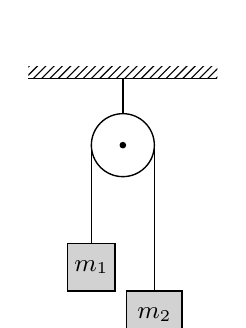
\begin{tikzpicture}[x=1cm,y=1cm,line width=0.5pt,>=Stealth,font=\small]
\draw (0,3.3)--(2.4,3.3); \fill[pattern=north east lines,draw=none] (0,3.3) rectangle (2.4,3.45); \draw (1.2,3.3)--(1.2,2.85); \draw[fill=white] (1.2,2.45) circle(0.4); \fill (1.2,2.45) circle(1.2pt);
\draw (0.8,2.45)--(0.8,1.2); \draw[fill=gray!35] (0.5,0.6) rectangle (1.1,1.2); \node at (0.8,0.9) {$m_1$};
\draw (1.6,2.45)--(1.6,0.6); \draw[fill=gray!35] (1.25,0.0) rectangle (1.95,0.6); \node at (1.6,0.3) {$m_2$};
\end{tikzpicture}\end{center}
\noindent\fbox{\begin{minipage}{0.64\linewidth}\vspace{4pt}\textbf{33.}\ Yuklarning tezlanişini (m/s$^2$) toping.\\[6pt]\textbf{34.}\ Ipning tarangligini (N) toping.\\[6pt]\textbf{35.}\ Blok öqiga ta’sir qiluvçi kuçni (N) toping.\vspace{4pt}\end{minipage}\vrule\hspace{6pt}\begin{minipage}{0.28\linewidth}\vspace{4pt}A)\ 2,5\\B)\ 5\\C)\ 37,5\\D)\ 40\\E)\ 75\\F)\ 80\vspace{4pt}\end{minipage}}\par\vspace{14pt}
\Needspace{9\baselineskip}
\noindent\textbf{36.}\ Qirrasining uzunligi 3 cm bölgan kub şaklidagi 3 ta muz bölagi asosining yuzasi 90 cm$^2$ bölgan, 107,1 g suv quyilgan silindrik idişda taşlandi. $\rho_{muz}=900$ kg/m$^3$.\par\smallskip
\medskip\noindent\textbf{a)\ Muzlar erib ketgandan söng suyuqlikning idiş tubiga beradigan bosimini (Pa) toping.}\par
\noindent\textit{Javob}: a)\ \blank\par
\medskip\noindent\textbf{b)\ Muzlar erib ketgandan söng suyuqlikning idiş tubiga beradigan bosim kuçini (N) hisoblang.}\par
\noindent\textit{Javob}: b)\ \blank\par
\medskip\noindent\textbf{Diqqat!} Javoblaringizni javoblar varaqasiga köçirib yozing.\par\vspace{10pt}
\Needspace{9\baselineskip}
\noindent\textbf{37.}\ Silindrik idişga teng massali suv va kerosin quyildi. Suyuqliklar ustunining umumiy balandligi 36 cm ga teng. $\rho_{kerosin}=800$ kg/m$^3$.\par\smallskip
\medskip\noindent\textbf{a)\ Suv ustunining balandligini (cm) aniqlang.}\par
\noindent\textit{Javob}: a)\ \blank\par
\medskip\noindent\textbf{b)\ Idiş tubidan 12 cm balandlikdagi nuqtada suyuqliklarning hosil qilgan umumiy bosimini (Pa) toping.}\par
\noindent\textit{Javob}: b)\ \blank\par
\medskip\noindent\textbf{Diqqat!} Javoblaringizni javoblar varaqasiga köçirib yozing.\par\vspace{10pt}
\Needspace{9\baselineskip}
\noindent\textbf{38.}\ Uzunligi 16 m, qiyalik burçagi $53^\circ$ bölgan silliq qiya tekislik tepasidan 2 kg massali jism sirpanib tuşdi. $\sin53^\circ=0,8$, $\cos53^\circ=0,6$.\par\smallskip
\medskip\noindent\textbf{a)\ Jismning qiya tekislik etagidagi tezligini (m/s) toping.}\par
\noindent\textit{Javob}: a)\ \blank\par
\medskip\noindent\textbf{b)\ Bu jarayonda oğirlik kuçining bajargan işini (J) toping.}\par
\noindent\textit{Javob}: b)\ \blank\par
\medskip\noindent\textbf{Diqqat!} Javoblaringizni javoblar varaqasiga köçirib yozing.\par\vspace{10pt}
\Needspace{9\baselineskip}
\noindent\textbf{39.}\ Bir atomli ideal gazga 75 J issiqlik berib, hajmi izobarik ravişda 2 marta oşirildi.\par\smallskip
\medskip\noindent\textbf{a)\ Bunda gazning absolyut temperaturasi qanday özgaradi?}\par
\noindent\textit{Javob}: a)\ \blank\par
\medskip\noindent\textbf{b)\ Gazning bajargan işini (J) aniqlang.}\par
\noindent\textit{Javob}: b)\ \blank\par
\medskip\noindent\textbf{Diqqat!} Javoblaringizni javoblar varaqasiga köçirib yozing.\par\vspace{10pt}
\Needspace{9\baselineskip}
\noindent\textbf{40.}\ Issiqlik siğimi 500 J/K bölgan idişda 25 $^\circ$C temperaturali 6 $\ell$ suv bor. Idişga $-15\,^\circ$C temperaturali 2 kg muz taşlandi. $c_{suv}=4200$ J/(kg$\cdot$K), $c_{muz}=2100$ J/(kg$\cdot$K), $\lambda_{muz}=330$ kJ/kg.\par\smallskip
\medskip\noindent\textbf{a)\ Natijaviy temperaturani ($^\circ$C) toping.}\par
\noindent\textit{Javob}: a)\ \blank\par
\medskip\noindent\textbf{b)\ Muzning olgan issiqlik miqdorini (kJ) aniqlang.}\par
\noindent\textit{Javob}: b)\ \blank\par
\medskip\noindent\textbf{Diqqat!} Javoblaringizni javoblar varaqasiga köçirib yozing.\par\vspace{10pt}
\Needspace{9\baselineskip}
\noindent\textbf{41.}\ Elektron induksiyasi $B$ bölgan magnit maydonga tik uçib kirdi va $r$ radiusli aylana böylab harakatlana boşladi. $m_e$ — zarraning massasi, $e$ — elementar zaryad.\par\smallskip
\medskip\noindent\textbf{a)\ Uning burçak tezligini aniqlang.}\par
\noindent\textit{Javob}: a)\ \blank\par
\medskip\noindent\textbf{b)\ Tezligini aniqlang.}\par
\noindent\textit{Javob}: b)\ \blank\par
\medskip\noindent\textbf{Diqqat!} Javoblaringizni javoblar varaqasiga köçirib yozing.\par\vspace{10pt}
\Needspace{9\baselineskip}
\noindent\textbf{42.}\ Maydon kuçlanganligi $E$ bölgan bir jinsli elektr maydonda harakatlanayotgan elektron $l$ masofaga köçib, $A$ nuqtadan $B$ nuqtaga yetib bordi (rasmda $AD\perp \vec E$).\par\smallskip
\begin{center}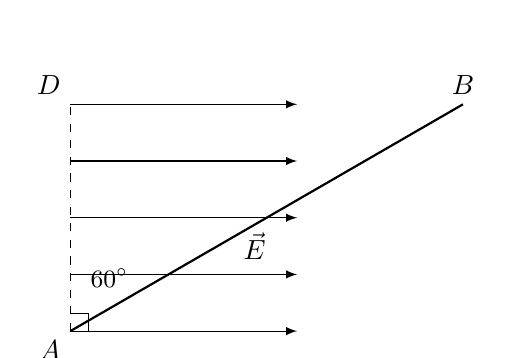
\begin{tikzpicture}[scale=0.9]\foreach \y in {0,0.8,1.6,2.4,3.2}{\draw[-latex] (0,\y)--(3.2,\y);}\draw (0.25,0)--(0.25,0.25)--(0,0.25);\draw[dashed] (0,0)--(0,3.2);\draw[thick] (0,0)--(5.54,3.2);\node[below left] at (0,0) {$A$};\node[above left] at (0,3.2) {$D$};\node[above] at (5.54,3.2) {$B$};\node at (2.6,1.2) {$\vec E$};\node at (0.55,0.75) {\small $60^\circ$};\end{tikzpicture}\end{center}
\medskip\noindent\textbf{a)\ Zarraning kinetik energiyasi qançaga özgarganini aniqlang.}\par
\noindent\textit{Javob}: a)\ \blank\par
\medskip\noindent\textbf{b)\ Zarra $ABDA$ yopiq yöl böylab köçirilganda elektr kuçlar bajaradigan işni aniqlang.}\par
\noindent\textit{Javob}: b)\ \blank\par
\medskip\noindent\textbf{Diqqat!} Javoblaringizni javoblar varaqasiga köçirib yozing.\par\vspace{10pt}
\Needspace{9\baselineskip}
\noindent\textbf{43.}\ Şişadagi nurning intensivligi 18 W/m$^2$ ga teng. $c=3\cdot10^8$ m/s.\par\smallskip
\medskip\noindent\textbf{a)\ Nurdagi elektromagnit maydon energiyasining ziçligini (J/m$^3$) aniqlang.}\par
\noindent\textit{Javob}: a)\ \blank\par
\medskip\noindent\textbf{b)\ Nur şişadagi absolyut qora sirtga tik tuşib töla yutilsa, sirtga beradigan bosimini (Pa) aniqlang.}\par
\noindent\textit{Javob}: b)\ \blank\par
\medskip\noindent\textbf{Diqqat!} Javoblaringizni javoblar varaqasiga köçirib yozing.\par\vspace{10pt}
\Needspace{9\baselineskip}
\noindent\textbf{44.}\ Quyoşning diametri $13,8\cdot10^{8}$ m ga, Yer bilan Quyoşn orasidagi masofa $1,5\cdot10^{11}$ m ga teng. Fokus masofasi 0,4 m bölgan Yerdagi linza ekranda Quyoşnning haqiqiy tasvirini hosil qilmoqda.\par\smallskip
\medskip\noindent\textbf{a)\ Tasvir bilan linza orasidagi masofani (mm) toping.}\par
\noindent\textit{Javob}: a)\ \blank\par
\medskip\noindent\textbf{b)\ Quyoşn tasvirining diametrini (mm) toping.}\par
\noindent\textit{Javob}: b)\ \blank\par
\medskip\noindent\textbf{Diqqat!} Javoblaringizni javoblar varaqasiga köçirib yozing.\par\vspace{10pt}
\Needspace{9\baselineskip}
\noindent\textbf{45.}\ Ğalayonlangan vodorod atomining ionlaşiş energiyasi 13,6 eV ga teng.\par\smallskip
\medskip\noindent\textbf{a)\ Atom fotonni yutib impuls momentini $3\hbar$ ga oşirsa, uning ionlaniş energiyasi (eV) nimaga teng bölişini aniqlang.}\par
\noindent\textit{Javob}: a)\ \blank\par
\medskip\noindent\textbf{b)\ Atom fotonni yutib impuls momentini $3\hbar$ ga oşirsa, undagi elektronning tezligi neça marta özgarişini aniqlang.}\par
\noindent\textit{Javob}: b)\ \blank\par
\medskip\noindent\textbf{Diqqat!} Javoblaringizni javoblar varaqasiga köçirib yozing.\par\vspace{10pt}
\end{document}